% 
%jff-notes
%
\documentclass[11pt]{article}
\usepackage[pdftex]{graphicx}
\usepackage{amssymb}
\usepackage{latexsym}
%\usepackage{relsize}
\usepackage{textcomp}
%processed for 10 pt 
%\documentstyle[epsf,psfig]{article}
%\documentstyle[epsf]{article}
\oddsidemargin 0pt
\topmargin -0.0cm
\textwidth 6.2in
\textheight 8.5in
\baselineskip 18pt
%\renewcommand{\baselinestretch} {1.5}
\newenvironment{nitemize}
   {\begin{list}{\begin{math}\bullet\end{math}}%
      {\setlength{\leftmargin}{5mm}
       \setlength{\topsep}{1mm}
       \setlength{\parsep}{0in}
       \setlength{\itemsep}{.7mm}}}%
   {\end{list}}

\newcommand{\fract}[2]{\frac{\textstyle #1}{\textstyle #2}}
\newcommand{\trans}[3]{#1 \stackrel{#2}{\longrightarrow} #3}
\newcommand{\notrans}[3]{#1 \stackrel{#2}{\not\! \longrightarrow} #3}
\bibliographystyle{plain}
\begin{document}
\title{A simple adsb plugin for SDRuno}
\author{
Jan van Katwijk\\
Lazy Chair Computing \\
The Netherlands\\
{\em J.vanKatwijk@gmail.com}}
%\date{}
\maketitle
%\baselineskip 22pt
\ \\
\ \\
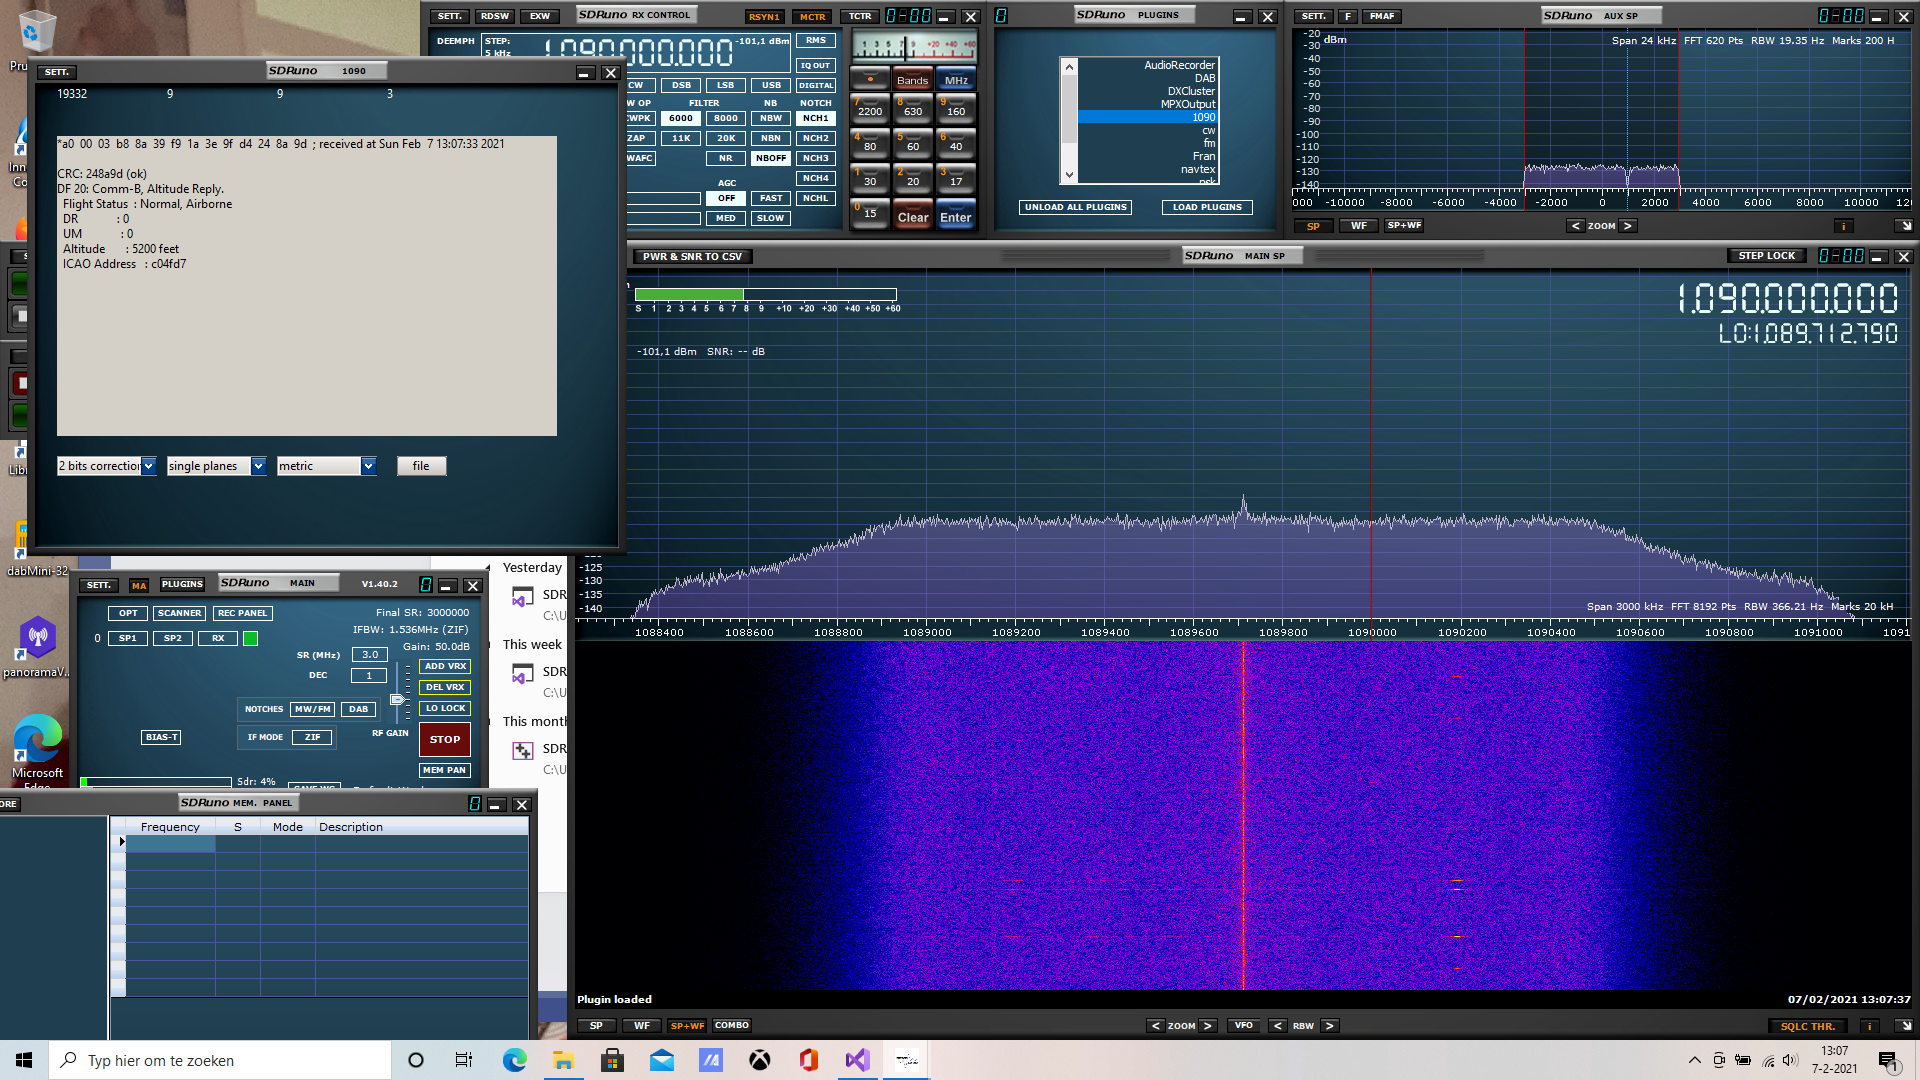
\includegraphics[width=140mm]{1090.png}
\ \\
\section{Introduction}
The SDRuno 1090 plugin is a simple plugin to for the reception and decoding
of adsb signals, as they are transmitted on 1090 MHz.

\section{Settings}
\subsection{Setting the samplerate}
The software uses internally asamplerate of 2400 KHz, and
assumes a setting of SDRuno on 3000 KHz  with a zero IF. Decimation
from 3000 KHz to 2400 KHz is done in the software.

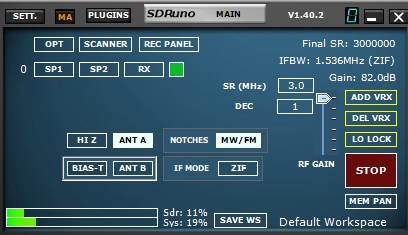
\includegraphics[width=100mm]{main-widget.png}

\subsection{Tuning}
Tuning is to 1090 MHz.

\subsection{Setting the map}
The plugin provides as option showing the planes on a map on a web browser.
In order to do so, one must place the file "gmap.html" in the {\em Documents}
folder in the user's home folder.

\section{The plugin}
The plugin widget  is shown in the picture

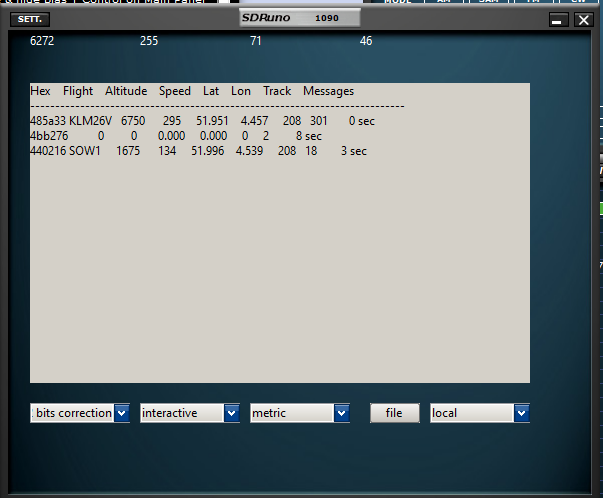
\includegraphics[width=100mm]{1090-widget.png}

The main widget contains three segments
\begin{itemize}
\item
the top row shows a number of figures, related to the received signal,
the first one is the number of potential good frames, the other ones
give the number of frames passing all tests and the number of 1 bit and
2 bit corrections applied;
\item the middle part will show either the messages as received or
a list of planes currently being visible, depending on the settings;
\item the bottom part contains 4 comboboxes and a button:
\begin{itemize}
\item the number of corrections. Default is set to no corrections,
one may select a one bit or two bit correction. Of course two bit correction takes some more CPU power than 1 bit correction or no correction;
\item the view. Selected is the interactive view, showing the list of planes
currently visible, the other view will display the messages as they are 
received and decoded;
\item metric;
\item the button with text {\em file}. If touched, a file menu will appear
with which a file can be selected. The data, as appearing in the interactive
screen, will be written to the file;
\item the selector labeled {\em local} gives a choice of leaving the
data local or making the data visible on a map.
If the {\em http on} option is chosen, a map and an indication
of the planes on it, can be made visible on a web browser through port 8080.
\end{itemize}
\end{itemize}
\end{document}

